\section{Cryptocurrencies correlation}
\label{sec:crypto_corr}

Blockchain was specifically designed to work with cryptocurrencies. In fact,
transactions works very well for transfer moneys from a user to another, while
every block works like an archive of transactions, allowing everyone to browse
the transaction history and check every money movement.

Miners for every transaction and for every block processed get a reward,
usually in the current cryptocurrency. This kind of reward mitigate attackers to
try to modify the Blockchain database to have an higher income.

Any user hold at least one \textbf{wallet}, that has a specific address. An
address is a random-generated token 26-35 alphanumeric characters long. Users
can have more than one wallet, and creating a new one it does not require any
authentication.

Moneys can be sent to non-existing wallets. This transaction is saved in the
chain and if someone create a wallet with the exact token it will redeem
the money.

\subsection{Privacy during transactions}

Due the fact that every transaction is broadcast to the network there is no
privacy about the transaction content. Everyone can see how much is sent to
other addresses. Many websites provide functionalities
\footnote{For example, \url{https://blockexplorer.com/} enable users to search
in the Bitcoin Blockchain.} that allows anyone to easily search data in a
Blockchain database. The ``real'' privacy that Blockchain offers is defined as
pseudo-privacy: everyone can see the details of any transaction, but it is very
difficult to know the people behind a payment, because the transfer is
identified only with wallets, that aren't physically linked to someone. There
are different studies \cite{guadamuz15} though that point out how it is
relatively easy for an attacker to discover user information thanks to payments
on online shops. An user could buy some goods from an online store with a
cryptocurrency, where she's registered with a username and password, linking
\textit{de facto} his identity with his wallet. Using a
\textit{mixer}\footnote{Mixers are online websites that splits the amount to
send to someone into different wallets, then they make fake transactions in
order obfuscate the sender to eventually send the money to the original
recipient.} could mitigate this problem, making more difficult to rebuild
history transactions for a single user.

\subsection{Account and Keys management}

User and account concepts do not exists in the Blockchain implementation per-se.
Therefore there is not any real account management, and no password
authentication. In its financial implementations, recovering a lost wallet is
usually almost impossible, because if the asymmetric keys are lost there is no
way to reclaim the transactions, hence to reclaim the money. This Blockchain
characteristic lead to money being locked-in forever into lost accounts in
cryptocurrencies.
It is important to note, by the way, that Blockchain implementations that differ
from Nakamoto's original idea could have account management, as for example
in\cite{azaria16} where the access to the Blockchain is regulated via prior
authentication, or in\cite{zhou16} where the authors added an authentication
layer to better manage Bitcoin accounts.

\begin{figure}[ht]
 \centering
 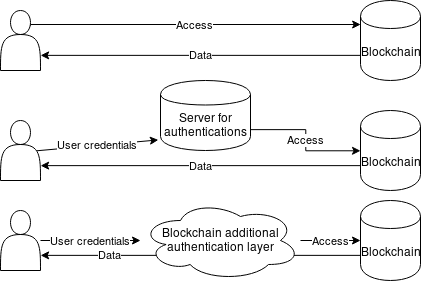
\includegraphics[scale=0.5]{authenticationMethods}
 \label{img:authMethods}
 \caption[Different ways to access a Blockchain database]{Different ways to
access a Blockchain database:
 \begin{enumerate*}[label=\arabic*)]
  \item without any extra authentication,
  \item via a separated server that manages user authentication,
  \item adding another verification layer.
 \end{enumerate*}}
\end{figure}

This highlight the importance for a user to keep a backup of her keys. Wallet
keys can be stored in different ways.

\paragraph{Digital Copy} One could make a simple digital copy of the key on a
digital storage (for example an USB key), but this would lead to expose the
keys to several vulnerabilities: first of all, the key could be stolen or lost.
Even having the keys in a physical media without any protection system is
dangerous: as explained in\cite{eskandari15}, an attacker could spread a
malware able to send to her copies of users' private keys. Encrypting the keys
would work only to mitigate theft attacks, but a malware could always be
shipped with a keylogger, nullifying this protection.

Coping the key online on some storage service or cloud will not enhance its
security either, because there is the possibility that the service provider
reads the user data, or that the service suffers an attack and leaks its
content.

\paragraph{Physical Copy} There is the possibility for currencies like Bitcoin
to print the wallet address and private key into a piece of paper. These system
though are not secure as they seems, because they are exposed, like media
storage, to the possibility of being stolen or the possibility to be lost.
Another threat is that the key could be easily seen and
copied~\cite{eskandari15}.


A possible solution to effectively protect the keys is using the multi-factor
authentication, that enhance the security, with a usability degradation.
